\let\negmedspace\undefined
\let\negthickspace\undefined
\documentclass[journal]{IEEEtran}
\usepackage[a5paper, margin=10mm, onecolumn]{geometry}
%\usepackage{lmodern} % Ensure lmodern is loaded for pdflatex
\usepackage{tfrupee} % Include tfrupee package

\setlength{\headheight}{1cm} % Set the height of the header box
\setlength{\headsep}{0mm}     % Set the distance between the header box and the top of the text

\usepackage{gvv-book}
\usepackage{gvv}
\usepackage{cite}
\usepackage{amsmath,amssymb,amsfonts,amsthm}
\usepackage{algorithmic}
\usepackage{graphicx}
\usepackage{textcomp}
\usepackage{xcolor}
\usepackage{txfonts}
\usepackage{listings}
\usepackage{enumitem}
\usepackage{mathtools}
\usepackage{gensymb}
\usepackage{comment}
\usepackage[breaklinks=true]{hyperref}
\usepackage{tkz-euclide} 
\usepackage{listings}
% \usepackage{gvv}                                        
\def\inputGnumericTable{}                                 
\usepackage[latin1]{inputenc}                                
\usepackage{color}                                            
\usepackage{array}                                            
\usepackage{longtable}                                       
\usepackage{calc}                                             
\usepackage{multirow}                                         
\usepackage{hhline}                                           
\usepackage{ifthen}                                           
\usepackage{lscape}

\usepackage{multicol}

% Marks the beginning of the document
\begin{document}
\bibliographystyle{IEEEtran}
\vspace{3cm}

\title{9.2.7}
\author{EE24BTECH11018 - Durgi Swaraj Sharma}
% \maketitle
% \newpage
% \bigskip
{\let\newpage\relax\maketitle}
\renewcommand{\thefigure}{\theenumi}
\renewcommand{\thetable}{\theenumi}

\textbf{Exercise 9.2} In each of the Exercises 1 to 10 verify that the given functions (explicit or implicit) is a solution of the corresponding differential equation:
\begin{align}
	7.\, xy = log y + C &: y^{\prime} = \frac{y^2}{1 - xy} \brak{xy \neq 1}
\end{align}
\subsection*{Theroretical solution}
\begin{align}
	\frac{dy}{dx} = \frac{y^2}{1 - xy} \brak{xy \neq 1}
\end{align}
Taking reciprocal,
\begin{align}
	\frac{dx}{dy} &= \frac{1 - xy}{y^2}\\
	\frac{dx}{dy} &= \frac{1}{y^2} - \frac{x}{y}
\end{align}
Rearranging the terms,
\begin{align}
	\frac{dx}{dy} + x\brak{\frac{1}{y}} &= \frac{1}{y^2}
\end{align}
We can apply the Integrating Factor method to solve this differential equation, 
\begin{align}
	\text{where}\, IF &= e^{\int{\frac{1}{y}dy}} = e^{ln\brak{y}} = y\\
	IF \cdot x &= \int{IF\cdot \frac{1}{y^2} } dy\\
	yx &= \int{y \frac{1}{y^2} }dy\\
	xy &= ln\brak{y} + C
\end{align}
We have theoretically verified that the given function is a solution to the given differential equation.

\subsection*{Numerical Solution}
We shall write computer programs that will give us an approximate solution to the differential equation, if we know the solution's starting point.\\
The following algorithm is the Finite Differences algorithm.
\begin{align*}
	\text{Let initial point be} \myvec{x_i, y_i}&\\
	\text{Set}\, x_0\leftarrow x_i, y_0\leftarrow y_i. \\\text{Let} \myvec{x_1, y_1}, \cdots, \myvec{x_n, y_n} \text{be approximate points on the solution curve.}&\\
	\text{Iterate:} \\y_{n+1} = y_{n} + h \cdot y_n^{\prime} \\ x_{n+1} = x_n + h.&
\end{align*}
The iteration step is derived from the Difference Equation which is given by,
\begin{align}
	\frac{dy}{dx} &\approx \frac{f\brak{x+h} -f\brak{x}}{h}\\ 
	\frac{dy}{dx} &\approx \frac{y_{i+1} - y_i}{h}
\end{align}
Rearranging,
\begin{align}
	y_{n+1} = y_n + \frac{dy}{dx} \, h
\end{align}
Due to the nature of our differential equation's finite difference, the Finite Differences algorithm is the same as Euler's method.\\
Applying this algorithm to our differential equation,
\begin{align}
	\text{Taking initial point \brak{\text{without loss of generality}} as} \myvec{5, 1}\\
	x_0\leftarrow 5, y_0\leftarrow 1\\
	\text{Iterate}\, x_{n+1} = x_n + h, y_{n+1} = y_n + h \cdot \frac{y_n^2}{1-x_ny_n}
\end{align}
Verifying this algorithm,
\begin{center} 
	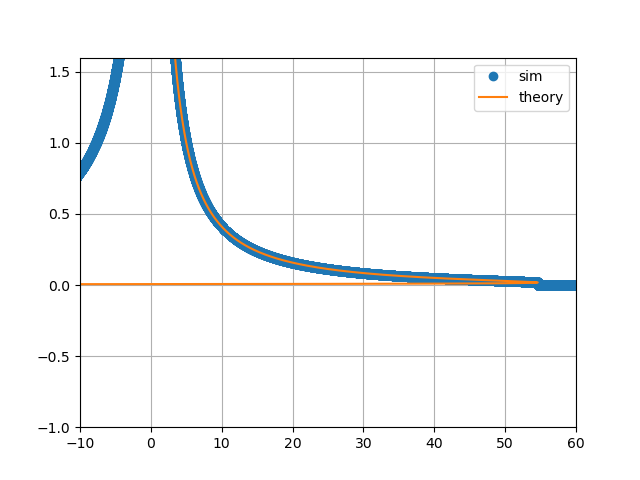
\includegraphics[width=\columnwidth]{/home/gvt1/sdcard/github/EE1003/Assignment1/figs/badEulersFull.png}  
	\captionof{figure}{Verification of our Finite Differences algorithm}
\end{center}
we can see that the simulation graph shows unusual behaviour. To fix this, we will apply the Finite Differences algorithm as follows,
\begin{align*}
	\text{Let initial point be} \myvec{x_i, y_i}&\\
	\text{Set}\, x_0\leftarrow x_i, y_0\leftarrow y_i. \\\text{Let} \myvec{x_1, y_1}, \cdots, \myvec{x_n, y_n} \text{be approximate points on the solution curve.}&\\
	\text{Iterate:}\\ x_{n+1} = x_{n} + h \cdot x_n^{\prime} \\ y_{n+1} = y_n + h.&
\end{align*}
This prevents our code from producing inaccurate results when $\frac{dy}{dx} \to \infty$.
\begin{center}
	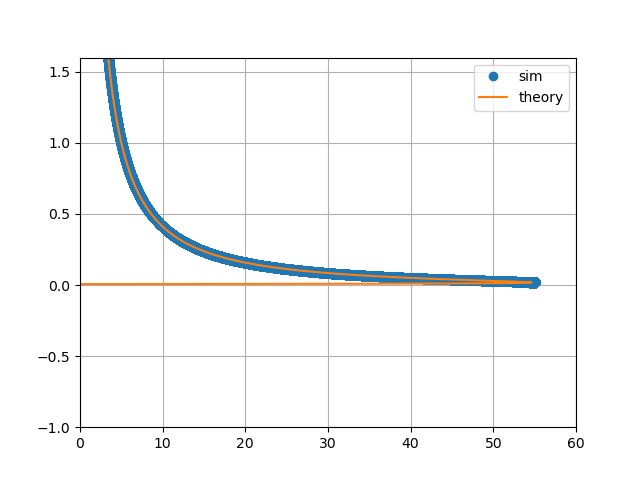
\includegraphics[width=\columnwidth]{/home/gvt1/sdcard/github/EE1003/Assignment1/figs/goodEulers.png}  
	\captionof{figure}{Verification after interchanging $x$ and $y$}
\end{center}
However, on oberving at a closer scale, we notice that the simulation strays away too quickly from the true values at crucial regions of the graph. 
\begin{center} 
	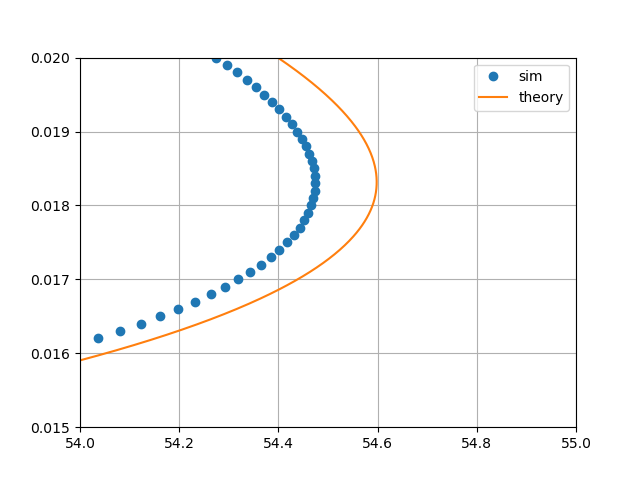
\includegraphics[width=\columnwidth]{/home/gvt1/sdcard/github/EE1003/Assignment1/figs/badEulers.png}  
	\captionof{figure}{Zoomed in section of the previous graph}
\end{center}
We will have to use an algorithm that converges fast enough to be useful in our case. 
One of these methods is the Improved Euler's method, which is as follows
\begin{align*}
	\text{Let initial point be} \myvec{x_i, y_i}&\\
	\text{Set}\, x_0 \leftarrow x_i, y_0 \leftarrow y_i. \\\text{Let} \myvec{x_1, y_1}, \cdots, \myvec{x_n, y_n} \text{be approximate points on the solution curve.}&\\
	\text{Iterate:} &\\
	k_1 = h \cdot y_n^{\prime}, \quad \text{where } y_n^{\prime} = f(x_n, y_n)& \\
	k_2 = h \cdot f\left(x_n + h, y_n + k_1\right)& \\
	y_{n+1} = y_n + \frac{1}{2} \cdot (k_1 + k_2)& \\
	x_{n+1} = x_n + h&
\end{align*}
Applying the same $x$ to $y$ switch we made to the previous approach and plotting, the result is
\begin{center} 
	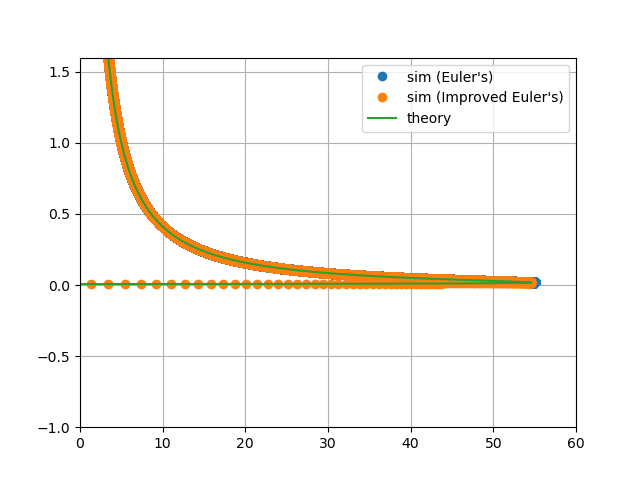
\includegraphics[width=\columnwidth]{/home/gvt1/sdcard/github/EE1003/Assignment1/figs/all.png}  
	\captionof{figure}{Verification of Improved Euler's method}
\end{center}
And a closer look:
\begin{center} 
	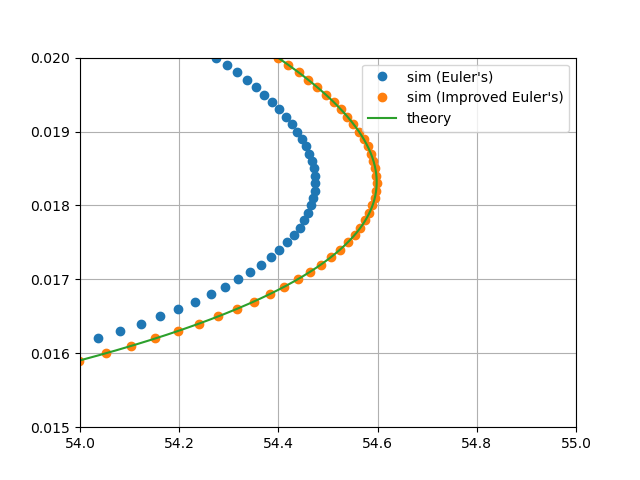
\includegraphics[width=\columnwidth]{/home/gvt1/sdcard/github/EE1003/Assignment1/figs/allZoomed.png}  
	\captionof{figure}{Zoomed in section of the previous graph}
\end{center}
Thus, we have numerically verified that $xy = log\brak{y} + C$ is a solution to the differential equation $\frac{dy}{dx} = \frac{y^2}{1-xy}$.
\end{document}
